%% =============================================================================
%% manuscript-anon.tex — The American Mathematical Monthly (anonymous review copy)
%% Title:    The Continuous-Coefficient Jensen Equation:
%%           How Real Mixing Weights Retire Regularity
%% Date:     2026-06-11  (review-panel revision)
%%
%% Compilation (TeX Live): run pdflatex twice. The references are a
%% hand-maintained thebibliography in Monthly house style; do NOT run BibTeX
%% (vancouver.bst is no longer part of the build).
%%
%% Class: MAA Monthly template (article + maa-monthly.sty).
%%
%% DOUBLE-BLIND SUBMISSION (Monthly policy):
%%   This file compiles TWO documents in sequence:
%%   (1) Title page with author details (page 1).
%%   (2) Anonymous manuscript body (pages 2+).
%%   To produce the ANONYMOUS-ONLY PDF, comment out the title-page
%%   block between the markers below and recompile.
%%
%% maa-monthly.sty already loads the following -- do NOT re-add them:
%%   times, pifont, graphicx, color,
%%   amsmath, amsthm, amsfonts, amssymb, url.
%% =============================================================================

\documentclass{article}
\usepackage{maa-monthly}

%% --- Additional packages not in maa-monthly.sty ---
\usepackage[utf8]{inputenc}     % UTF-8 source encoding
\usepackage[T1]{fontenc}        % Type-1 output encoding
\usepackage{microtype}          % improved microtypography (safe with Times)
\usepackage{booktabs}           % \toprule, \midrule, \bottomrule
\usepackage{array}              % extended column specifiers in tables
\usepackage{tabularx}           % X column type for proportional-width tables
\usepackage{tikz}               % figures (load diagram, mechanism, resolution axis)

%% --- Theorem environments (following the Monthly template exactly) ---
\theoremstyle{plain}
\newtheorem{theorem}{Theorem}
\newtheorem{proposition}[theorem]{Proposition}
\newtheorem{lemma}[theorem]{Lemma}
\newtheorem{corollary}[theorem]{Corollary}

\theoremstyle{definition}
\newtheorem{definition}[theorem]{Definition}
\newtheorem{remark}[theorem]{Remark}

%% --- Math abbreviations ---
\newcommand{\R}{\mathbb{R}}
\newcommand{\Q}{\mathbb{Q}}
\newcommand{\E}{\mathbb{E}}

%% =============================================================================
\begin{document}

%% ---------------------------------------------------------------------------
%% TITLE PAGE WITH AUTHOR DETAILS — REMOVED FROM THIS ANONYMOUS REVIEW COPY.
%% Author name, affiliation, contact, and biography live ONLY in the
%% "with author details" file (manuscript.tex), never in this anonymous source.
%% Do not paste any identifying information below this line.
%% ---------------------------------------------------------------------------

%% ---------------------------------------------------------------------------
%% ANONYMOUS MANUSCRIPT BODY (double-blind: no author name below this line)
%% ---------------------------------------------------------------------------

\title{The Continuous-Coefficient Jensen Equation:\\
       How Real Mixing Weights Retire Regularity}

%% Running head: abbreviated title, ≤50 characters.
\markright{Continuous-coefficient Jensen equation}

%% DO NOT fill in author names until the PROVISIONAL ACCEPT letter.
%% Monthly submissions are DOUBLE BLIND.
\author{}

\maketitle

%% ---------------------------------------------------------------------------
%% ABSTRACT
%% Guidelines: ≤250 words; entice the reader; minimize notation;
%%             highlight concepts, not mechanics.
%% ---------------------------------------------------------------------------
\begin{abstract}
Jensen's inequality is a workhorse of analysis: for every concave
function~$G$ and random variable~$\xi$ on an interval,
$\E[G(\xi)]\le G(\E[\xi])$. What if equality is forced for every
two-point distribution\,---\,that is,
$p\,G(u_1)+(1-p)\,G(u_2)=G(p\,u_1+(1-p)\,u_2)$ for all $u_1,u_2$ in
the interval and all weights $p\in[0,1]$? Must $G$ be affine?

Yes. The proof is one line\,---\,substitute $u_1=M$, $u_2=0$, $p=v/M$
and read $G(v)$ off the chord through $(0,G(0))$ and
$(M,G(M))$\,---\,and it needs no regularity hypothesis on~$G$: no
continuity, measurability, monotonicity, or boundedness.

The contrast with rational weights is sharp. The $p=\tfrac12$ case is
equivalent to Cauchy's additive equation, which admits wildly
pathological non-affine solutions (Hamel, 1905) unless a regularity
hypothesis intervenes. Classical analysis from Cauchy (1821) to
Kestelman (1947) cataloged the minimal tameness conditions that rule
the pathology out, and the conditions became standard baggage in
functional-equation arguments\,---\,carried even where the
continuous-coefficient equation is in play and none of the baggage is
needed.

This expository article makes the asymmetry explicit. We catalog which
classical regularity hypotheses become vestigial under the
continuous-coefficient equation, explain why (the Hamel pathology
lives at irrational weights, exactly where the equation now
tests~$G$), and give a diagnostic separating the saturated-Jensen
settings where the hypotheses are vestigial from the more common
settings where they remain load-bearing. The same five hypotheses
appear on both sides of the line: indispensable in the axiomatic
characterization of Shannon entropy, vestigial in a calibration
computation on an atomless space.
\end{abstract}

\vspace{8px}

\noindent\textbf{Keywords:} Jensen equation, Cauchy equation, Hamel basis,
functional equation, regularity hypothesis

\vspace{4px}

\noindent\textbf{MSC 2020:} Primary 39B22; Secondary 26B25, 91B16, 94A17

\vspace{8px}

%% =============================================================================
\section{Introduction.}
\label{sec:intro}

One of the most serviceable inequalities in mathematics---Jensen's
inequality~\cite{Jensen1906}, $\E[G(\xi)]\le G(\E[\xi])$ for concave~$G$---raises an
immediate follow-up: when does equality hold for \emph{every} two-point
distribution supported on a given interval? The equation expressing
universal two-point equality,
\begin{equation}
p\,G(u_1)+(1-p)\,G(u_2) \;=\; G\bigl(p\,u_1+(1-p)\,u_2\bigr)
\qquad (u_1,u_2\in I,\ p\in[0,1]),
\tag{$\star$}\label{eq:star}
\end{equation}
imposed on a function $G\colon I\to\R$ on a real interval $I$, has
at least three forms in classical analysis. The three forms are easily
conflated---and have been, on and off, for a century---with consequences
for both the foundational theory and the modern applied literature where
the equation surfaces.

\subsection{Three forms of the equation.}

The \emph{discrete-coefficient} Jensen equation,
\begin{equation}
G\!\left(\tfrac{u_1+u_2}{2}\right) \;=\; \tfrac{G(u_1)+G(u_2)}{2},
\tag{$J_2$}\label{eq:J2}
\end{equation}
is the $p=\tfrac{1}{2}$ specialization of~\eqref{eq:star}. Setting
$f(x):=G(x)-G(0)$, the equation~\eqref{eq:J2} is equivalent on a
translate of~$I$ to Cauchy's additive equation $f(x+y)=f(x)+f(y)$.
Cauchy's equation inherits a full apparatus of pathological solutions:
without measurability, monotonicity, boundedness on a set of positive
Lebesgue measure, or another regularity hypothesis, the equation admits
non-affine solutions constructed via a \emph{Hamel basis}---a basis
of~$\R$ as a $\Q$-vector space, whose existence requires the axiom of
choice. The classical pathological-solution apparatus is the work of
Hamel~\cite{Hamel1905}; the regularity hypotheses sufficient to recover
affineness were cataloged by Cauchy~\cite{Cauchy1821},
Darboux~\cite{Darboux1875,Darboux1880}, Sierpi\'nski~\cite{Sierpinski1920},
Kormes~\cite{Kormes1926}, Ostrowski~\cite{Ostrowski1929}, and
Kestelman~\cite{Kestelman1947}, with Steinhaus's difference-set
theorem~\cite{Steinhaus1920} supplying the tool behind the modern
proofs of the measure-theoretic entries; Reem~\cite{Reem2017} surveys
the catalog.

The \emph{rational-coefficient} Jensen equation,
\begin{multline}
p\,G(u_1)+(1-p)\,G(u_2)
  \;=\; G\bigl(p\,u_1+(1-p)\,u_2\bigr) \\
  (u_1,u_2\in I,\quad p\in[0,1]\cap\Q),
\tag{$J_\Q$}\label{eq:JQ}
\end{multline}
strengthens~\eqref{eq:J2} but does not escape its pathology. Cauchy
additivity entails $\Q$-homogeneity---$f(qx)=qf(x)$ for every $q\in\Q$
and $x\in\R$---by an elementary induction on positive integers, sign
reversal for negatives, and the inverse-of-multiplication argument for
$1/n$. Combining additivity with $\Q$-homogeneity
returns~\eqref{eq:JQ} for~$f$, hence for~$G$. So \eqref{eq:JQ},
\eqref{eq:J2}, and Cauchy's equation share the same solution class up to
constants, and all three inherit the Hamel-basis pathology.

The \emph{continuous-coefficient} form~\eqref{eq:star}, by contrast, is
fundamentally different. The strengthening from $\Q$ to $\R$ in the
range of~$p$ is \emph{genuine}. As we will see, \eqref{eq:star} does not
admit any Hamel pathology: the pathology cannot survive at irrational~$p$,
and the continuous-coefficient equation tests~$G$ at every irrational.
This is the subject of the paper.

\subsection{The main result.}

\begin{theorem}\label{thm:main}
Let $M>0$ and let $G\colon[0,M]\to\R$ satisfy~\eqref{eq:star} for every
$u_1,u_2\in[0,M]$ and every $p\in[0,1]$. Then $G$ is affine on $[0,M]$:
\[
G(v) \;=\; \frac{G(M)-G(0)}{M}\,v + G(0), \quad v\in[0,M].
\]
\end{theorem}

The hypothesis list deserves a second look: no regularity of any
kind---continuity, measurability, monotonicity, or boundedness---is
assumed of~$G$. The proof is one line: a substitution into~\eqref{eq:star} that pins
$G(v)$ on the straight line through the endpoints $(0,G(0))$ and
$(M,G(M))$.
We give it in Section~\ref{sec:proof} and use the remainder of the paper
to articulate what it means.

\subsection{The historical detour and the structural moral.}
\label{ssec:detour}

Theorem~\ref{thm:main} is elementary. The underlying substitution
technique is folklore in functional equations: Acz\'el's
\cite[\S2.1.4]{Aczel1966} contains a dyadic precursor proved (with a
continuity hypothesis) by a dyadic-induction argument. The precise
statement of Theorem~\ref{thm:main}\,---\,continuous coefficients
$p\in[0,1]$, no regularity hypothesis on~$G$\,---\,does not appear in
this exact form in the standard references the author consulted; it is
recorded here because the recurrence pattern of
Section~\ref{sec:recurrence} needs it as a separable lemma. The
contribution of the present paper is in three parts:
\begin{itemize}
\item \emph{The explicit dictionary} (Section~\ref{sec:dictionary}) of
  classical regularity hypotheses on~$G$\,---\,continuity, measurability,
  monotonicity, boundedness on a set of positive measure, and
  boundedness on the interval\,---\,each of which is required to force
  affineness for~\eqref{eq:J2} but becomes \emph{vestigial}
  under~\eqref{eq:star}, together with the structural mechanism (the
  Hamel pathology lives at irrational~$p$, exactly where
  \eqref{eq:star}'s continuous coefficient closes the door).

\item \emph{The strict-minimum hypothesis}
  (Section~\ref{ssec:weak})---the
  equation~\eqref{eq:star} at a single endpoint configuration already
  suffices.

\item \emph{The diagnostic} (Section~\ref{sec:recurrence}) for
  distinguishing saturated-Jensen derivations that genuinely produce
  the continuous-coefficient equation\,---\,where the dictionary's
  regularity hypotheses are vestigial\,---\,from those that produce a
  rational-coefficient relative, an additive function into a bounded
  codomain, a Cauchy relative with a non-affine target, or no
  real-valued unknown at all (the zeroth gate). In the
  latter cases the same hypotheses\,---\,or an existence axiom prior
  to them\,---\,are load-bearing; the
  misclassification runs in both directions, and we give examples of
  each.
\end{itemize}

Stylistically, this article foregrounds one part of Jensen-equation
theory: the regime in which the continuous-coefficient form needs no
regularity assumption on the function. That emphasis is ours; Kuczma's
monograph~\cite{Kuczma2009} is the canonical modern reference for the
Cauchy and Jensen equations \emph{as a whole}, treating both the
regularity catalog\,---\,which hypotheses force affineness\,---\,and the
regularity-free structural theory.
The substitution that closes~\eqref{eq:star} is one of the simplest
observations in that tradition; what justifies writing it down is the
dictionary, the structural mechanism, and the survey of applied
recurrences.

The classical detour through Hamel and the Polish school answered a
perfectly natural question---\emph{what regularity hypothesis suffices
for \eqref{eq:J2}$\Rightarrow$affine?}---but a \emph{different}
question from the one that matters for many modern applications. The
applied derivation does not produce \eqref{eq:J2} or \eqref{eq:JQ};
it produces \eqref{eq:star} as a saturated identity, and the one-line
substitution of Section~\ref{sec:proof} is the right closure tool. The
dictionary of Section~\ref{sec:dictionary} makes explicit which classical
regularity hypotheses become vestigial in this transition.

The pattern\,---\,a continuum built into the model retiring a
classical hypothesis\,---\,has a distinguished ancestor. In exchange
economies with an atomless continuum of traders, Aumann showed that
convexity of preferences becomes unnecessary~\cite{Aumann1964},
Lyapunov-type convexity supplying for free what the hypothesis used to
buy. The present article records the same phenomenon one level down, at
the level of a single functional equation on an interval.

\paragraph{Terminology.}
Throughout the paper we refer to the substitution $u_1=M$, $u_2=0$,
$p=v/M$ in~\eqref{eq:star}\,---\,by which $G(v)$ is read off the straight
line through the endpoints $(0,G(0))$ and $(M,G(M))$\,---\,as the
\emph{endpoint substitution}. The descriptive
label is our convenience, adopted for brevity in repeated reference
rather than as a claim of established terminology.

%% =============================================================================
\section{The result and its proof.}
\label{sec:proof}

\begin{proof}[Proof of Theorem~\ref{thm:main}]
Fix $v\in[0,M]$. Set
\[
u_1 := M, \qquad u_2 := 0, \qquad p := \frac{v}{M}.
\]
The constraints of~\eqref{eq:star} are satisfied: $u_1=M\in[0,M]$,
$u_2=0\in[0,M]$, and $p=v/M\in[0,1]$ since $v\in[0,M]$.
Substituting into~\eqref{eq:star},
\[
\frac{v}{M}\,G(M)+\left(1-\frac{v}{M}\right)G(0)
\;=\;
G\!\left(\frac{v}{M}\cdot M+\left(1-\frac{v}{M}\right)\cdot 0\right)
\;=\; G(v).
\]
Rearranging yields $G(v)=G(0)+\bigl(G(M)-G(0)\bigr)\,v/M$.
\end{proof}

The endpoint substitution pins $G(v)$ on the straight line from
$(0,G(0))$ to $(M,G(M))$ for every $v\in[0,M]$. Since this determines
$G(v)$ at every~$v$, the function~$G$ is fully determined by its values
at the two endpoints\,---\,it is exactly the affine function joining them.

\begin{corollary}\label{cor:regularity}
Under the hypotheses of Theorem~\ref{thm:main}, $G$ is in particular
continuous, monotone, Lipschitz, absolutely continuous, and
Lebesgue measurable on $[0,M]$.
\end{corollary}

\begin{proof}
Every affine function $G(v)=av+b$ on a bounded interval is differentiable
with constant derivative $G'=a$, hence continuous; non-decreasing if
$a\ge0$ and non-increasing if $a\le0$; Lipschitz with constant~$|a|$;
absolutely continuous; and Borel-measurable, hence Lebesgue-measurable.
\end{proof}

The order of inference matters and is worth stating explicitly. Under
\eqref{eq:star}, the regularity properties of~$G$ are the
\emph{conclusion}, not the hypothesis. Each regularity hypothesis one
might be tempted to assume---continuity, monotonicity, boundedness,
measurability---is automatically satisfied by any solution
of~\eqref{eq:star}. The continuous-coefficient equation supplies its own
regularity from within; no external regularity hypothesis is needed.

This is what makes the continuous-coefficient case structurally different
from the discrete-coefficient case~\eqref{eq:J2}, where some regularity
hypothesis \emph{is} required to rule out the Hamel pathology. We now
examine the difference in detail.

%% =============================================================================
\section{The dictionary of vestigial regularity hypotheses.}
\label{sec:dictionary}

\subsection{The dictionary.}
\label{ssec:dict-table}

We place side-by-side the discrete-coefficient equation~\eqref{eq:J2}
and the continuous-coefficient equation~\eqref{eq:star}, and ask which
regularity hypotheses on~$G$ are \emph{required} to force affineness
for each. Table~\ref{tab:dictionary} lists these hypotheses side-by-side,
and Figure~\ref{fig:dictionary} draws the comparison as a load
diagram: five classical hypotheses, each individually strong enough
to carry the conclusion for~\eqref{eq:J2}, and the same conclusion
for~\eqref{eq:star} carried by the bare equation, every strut
removed. The caption of Figure~\ref{fig:dictionary} records the standard historical attribution of
each strut. (For a modern textbook treatment of the regularity
catalog for~\eqref{eq:J2} we refer the reader to
Kuczma~\cite[\S13.2]{Kuczma2009}.)

\begin{figure}[ht]
\centering
\resizebox{\linewidth}{!}{%
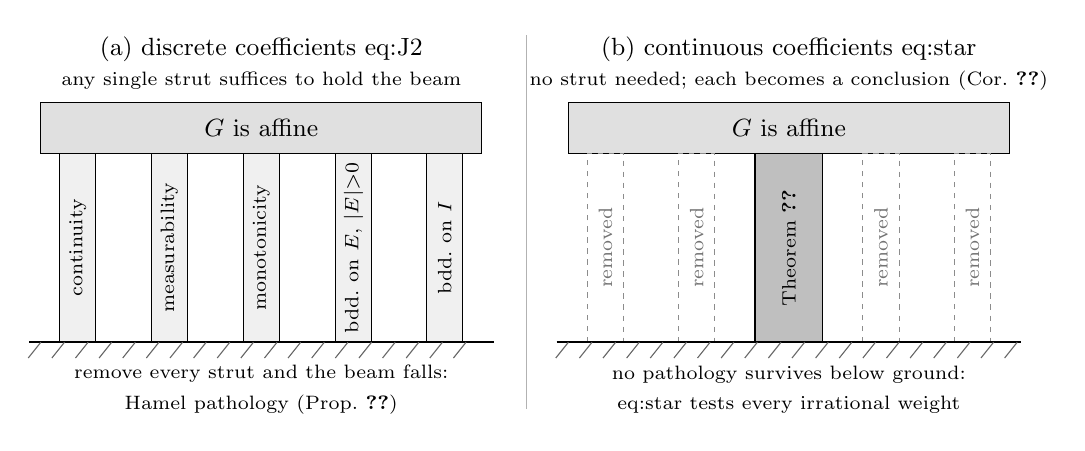
\begin{tikzpicture}[x=1cm,y=1cm]
% ---------------- panel (a): (J_2), rational weights ----------------
\node at (2.95,4.62) {\small (a) discrete coefficients \eqref{eq:J2}};
\node at (2.95,4.22) {\scriptsize any single strut suffices to hold the beam};
\fill[black!12] (0.15,3.30) rectangle (5.75,3.95);
\draw (0.15,3.30) rectangle (5.75,3.95);
\node at (2.95,3.625) {\small $G$ is affine};
% struts
\foreach \cx/\lab in {0.62/{continuity}, 1.78/{measurability},
  2.95/{monotonicity}, 4.12/{bdd.\ on $E$, $|E|{>}0$}, 5.28/{bdd.\ on $I$}}{
  \fill[black!6] (\cx-0.23,0.90) rectangle (\cx+0.23,3.30);
  \draw (\cx-0.23,0.90) rectangle (\cx+0.23,3.30);
  \node[rotate=90] at (\cx,2.10) {\scriptsize \lab};
}
% ground + hatching
\draw[thick] (0,0.90) -- (5.9,0.90);
\foreach \x in {0.15,0.45,...,5.85}{\draw[black!60] (\x,0.90) -- (\x-0.16,0.70);}
\node[align=center] at (2.95,0.30)
  {\scriptsize remove every strut and the beam falls:\\[-1pt]
   \scriptsize Hamel pathology (Prop.~\ref{prop:JQ-pathology})};
% ---------------- divider ----------------
\draw[black!30] (6.32,0.05) -- (6.32,4.80);
% ---------------- panel (b): (star), real weights ----------------
\node at (9.65,4.62) {\small (b) continuous coefficients \eqref{eq:star}};
\node at (9.65,4.22) {\scriptsize no strut needed; each becomes a conclusion (Cor.~\ref{cor:regularity})};
\fill[black!12] (6.85,3.30) rectangle (12.45,3.95);
\draw (6.85,3.30) rectangle (12.45,3.95);
\node at (9.65,3.625) {\small $G$ is affine};
% ghost struts (removed)
\foreach \cx in {7.32, 8.48, 10.82, 11.98}{
  \draw[black!45, dash pattern=on 2pt off 2pt] (\cx-0.23,0.90) rectangle (\cx+0.23,3.30);
}
\node[black!55, rotate=90] at (7.32,2.10) {\scriptsize removed};
\node[black!55, rotate=90] at (8.48,2.10) {\scriptsize removed};
\node[black!55, rotate=90] at (10.82,2.10) {\scriptsize removed};
\node[black!55, rotate=90] at (11.98,2.10) {\scriptsize removed};
% pedestal: the equation itself
\fill[black!25] (9.22,0.90) rectangle (10.08,3.30);
\draw (9.22,0.90) rectangle (10.08,3.30);
\node[rotate=90] at (9.65,2.10) {\scriptsize Theorem~\ref{thm:main}};
% ground + hatching
\draw[thick] (6.7,0.90) -- (12.6,0.90);
\foreach \x in {6.85,7.15,...,12.55}{\draw[black!60] (\x,0.90) -- (\x-0.16,0.70);}
\node[align=center] at (9.65,0.30)
  {\scriptsize no pathology survives below ground:\\[-1pt]
   \scriptsize \eqref{eq:star} tests every irrational weight};
\end{tikzpicture}%
}
\caption{The dictionary of vestigial regularity hypotheses, drawn as a
load diagram. (a)~Under the discrete-coefficient
equation~\eqref{eq:J2}, the conclusion ``$G$ is affine'' must be
carried by a regularity strut, and any single one suffices: continuity
(Cauchy~\cite{Cauchy1821}), measurability
(Sierpi\'nski~\cite{Sierpinski1920}), monotonicity
(Darboux~\cite{Darboux1875}), boundedness on a set of positive measure
(Kormes~\cite{Kormes1926}; one-sided bounds suffice,
Ostrowski~\cite{Ostrowski1929}, Kestelman~\cite{Kestelman1947}), or
boundedness on the interval (Darboux~\cite{Darboux1880}). Remove them
all and the beam falls: the Hamel-basis pathology~\cite{Hamel1905}
supplies a non-affine solution (Proposition~\ref{prop:JQ-pathology}).
Steinhaus's difference-set theorem~\cite{Steinhaus1920} powers the
modern proofs of the two measure-theoretic struts but is a tool, not a
strut; for the historical catalog see Reem~\cite{Reem2017} and
Kuczma~\cite[\S13.2]{Kuczma2009}. (b)~Under the continuous-coefficient
equation~\eqref{eq:star} the bare equation carries the load
(Theorem~\ref{thm:main}); every strut becomes a conclusion rather than
a hypothesis (Corollary~\ref{cor:regularity}), and no pathology
survives below ground, because~\eqref{eq:star} tests every irrational
weight.}
\label{fig:dictionary}
\end{figure}

\begin{table}[ht]
\renewcommand{\arraystretch}{1.4}
\centering
\begin{tabularx}{\linewidth}{@{} >{\raggedright\arraybackslash}X
  >{\raggedright\arraybackslash}X
  >{\raggedright\arraybackslash}X @{}}
\toprule
\textbf{Hypothesis on $G$} &
\textbf{For \eqref{eq:J2}$\Rightarrow$affine?} &
\textbf{For \eqref{eq:star}$\Rightarrow$affine?} \\
\midrule
\textbf{Continuity on $I$}: $G$ is continuous at every $v\in I$.
  & Yes, suffices (Cauchy~\cite{Cauchy1821}).
  & \textbf{No}---it is the \emph{conclusion} (Corollary~\ref{cor:regularity}). \\
\midrule
\textbf{Measurability on $I$}: $G$ is Lebesgue- or Borel-measurable on~$I$.
  & Yes, suffices (Sierpi\'nski~\cite{Sierpinski1920}).
  & \textbf{No}---same. \\
\midrule
\textbf{Monotonicity on $I$}: $G$ is non-decreasing or non-increasing on~$I$.
  & Yes, suffices (Darboux~\cite{Darboux1875}).
  & \textbf{No}---same. \\
\midrule
\textbf{Boundedness on a set of positive measure}: $G$ is bounded on some
  Lebesgue-measurable $E\subseteq I$ with $|E|>0$.
  & Yes, suffices (Kormes~\cite{Kormes1926}; bounded on one side
    suffices, Ostrowski~\cite{Ostrowski1929},
    Kestelman~\cite{Kestelman1947}).
  & \textbf{No}---same. \\
\midrule
\textbf{Boundedness on $I$}: $G$ is bounded on all of~$I$.
  & Yes, suffices (Darboux~\cite{Darboux1880}).
  & \textbf{No}---same. \\
\midrule
\textbf{None}: no regularity hypothesis at all.
  & \textbf{Insufficient}---Hamel-basis pathology~\cite{Hamel1905}.
  & \textbf{Sufficient}---Theorem~\ref{thm:main}. \\
\bottomrule
\end{tabularx}
\caption{Regularity hypotheses on $G$. Column~2 records which hypotheses
are classically required to force affineness for the
discrete-coefficient equation~\eqref{eq:J2}. Column~3 records their
status under the continuous-coefficient equation~\eqref{eq:star}.
Steinhaus's difference-set theorem~\cite{Steinhaus1920} powers the
modern proofs of the two measure-theoretic rows but is itself a tool
rather than a regularity result; for the historical catalog see
Reem~\cite{Reem2017} and Kuczma~\cite[\S13.2]{Kuczma2009}.}
\label{tab:dictionary}
\end{table}
% --- end former Table 1 ---

The ground line is the point of the figure. With \textbf{no
hypothesis at all}, the beam falls for~\eqref{eq:J2}: there exists a
non-affine, non-measurable, unbounded additive function
on~$\R$---the classical Hamel-basis pathology~\cite{Hamel1905}---that
supplies a non-affine solution of~\eqref{eq:J2}. Conversely,
\textbf{no hypothesis is needed} for~\eqref{eq:star}:
Theorem~\ref{thm:main}'s endpoint substitution closes the proof at
the level of the bare functional equation.

The five struts tell a complementary story. For~\eqref{eq:J2},
\emph{some} strut is required; otherwise the Hamel pathology
survives. For~\eqref{eq:star}, \emph{none} is required---and yet each
is automatically satisfied by any solution
(Corollary~\ref{cor:regularity}). Each hypothesis is, in the
dictionary's terminology, \emph{vestigial}: classically required
for~\eqref{eq:J2}, classically expected for~\eqref{eq:star}, but in
fact unnecessary for~\eqref{eq:star}.

\subsection{The structural mechanism.}
\label{ssec:mechanism}

Why does the Hamel pathology fail to apply to~\eqref{eq:star}? The
mechanism is direct and illuminating.

A Hamel-basis pathological solution $G$ of Cauchy's equation on~$\R$ is
$\Q$-linear: $G(0)=0$ and $G(qx)=q\,G(x)$ for every $q\in\Q$ and
$x\in\R$. By design, $G$ is \emph{not} $\R$-linear: there exists an
irrational $r\in\R$ and an $x\in\R$ such that $G(rx)\ne r\,G(x)$.

The straight-line identity in~\eqref{eq:star} at the configuration $u_1=M$,
$u_2=0$ reads
\begin{equation}
p\,G(M)+(1-p)\,G(0) \;=\; G(p\,M).
\tag{$\star_0$}\label{eq:star0}
\end{equation}
For a Hamel-pathological $G$ (so $G(0)=0$), \eqref{eq:star0} becomes
$p\,G(M)=G(p\,M)$---exactly the $\R$-linearity assertion for~$G$ at the
pair $(M,p)$. By $\Q$-linearity of~$G$, this holds for every $p\in\Q$.
By the failure of $\R$-linearity, it \emph{fails} at some irrational~$p$.
So the Hamel-pathological $G$ satisfies~\eqref{eq:JQ} (every rational
coefficient is OK) but violates~\eqref{eq:star} at every irrational~$p$
where the $\R$-linearity defect appears.

The structural point is one sentence:

\begin{quote}
\textbf{The Hamel pathology lives at irrational $p$; the
continuous-coefficient equation~\eqref{eq:star} forecloses on it there.}
\end{quote}

Figure~\ref{fig:mechanism} draws both halves of that sentence.

\begin{figure}[ht]
\centering
\resizebox{\linewidth}{!}{%
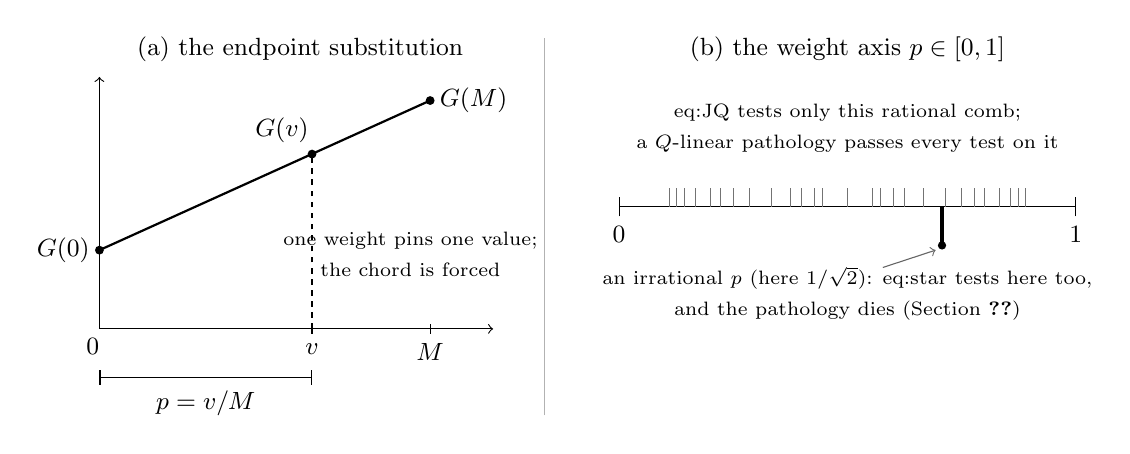
\begin{tikzpicture}[x=1cm,y=1cm]
% ---------------- panel (a): endpoint substitution ----------------
\node at (2.55,3.55) {\small (a) the endpoint substitution};
\draw[->] (0,0) -- (5.0,0);
\draw[->] (0,0) -- (0,3.2);
\draw (4.2,0.06) -- (4.2,-0.06) node[below] {\small $M$};
\draw (2.7,0.06) -- (2.7,-0.06) node[below] {\small $v$};
\node[below left] at (0.12,0) {\small $0$};
\draw[thick] (0,1.0) -- (4.2,2.9);
\fill (0,1.0) circle (1.6pt) node[left] {\small $G(0)$};
\fill (4.2,2.9) circle (1.6pt) node[right] {\small $G(M)$};
\draw[dash pattern=on 2pt off 2pt] (2.7,0) -- (2.7,2.22);
\fill (2.7,2.22) circle (1.6pt);
\node[above left] at (2.78,2.24) {\small $G(v)$};
\draw[|-|] (0,-0.62) -- (2.7,-0.62);
\node at (1.35,-0.95) {\small $p=v/M$};
\node[align=center] at (3.95,0.95)
  {\scriptsize one weight pins one value;\\[-1pt]\scriptsize the chord is forced};
% ---------------- divider ----------------
\draw[black!30] (5.65,-1.1) -- (5.65,3.7);
% ---------------- panel (b): the weight axis ----------------
\node at (9.5,3.55) {\small (b) the weight axis $p\in[0,1]$};
\draw (6.6,1.55) -- (12.4,1.55);
\draw (6.6,1.43) -- (6.6,1.67) node[below=7pt] {\small $0$};
\draw (12.4,1.43) -- (12.4,1.67) node[below=7pt] {\small $1$};
\draw[black!55] (7.244,1.55) -- (7.244,1.79);
\draw[black!55] (7.325,1.55) -- (7.325,1.79);
\draw[black!55] (7.429,1.55) -- (7.429,1.79);
\draw[black!55] (7.567,1.55) -- (7.567,1.79);
\draw[black!55] (7.760,1.55) -- (7.760,1.79);
\draw[black!55] (7.889,1.55) -- (7.889,1.79);
\draw[black!55] (8.050,1.55) -- (8.050,1.79);
\draw[black!55] (8.257,1.55) -- (8.257,1.79);
\draw[black!55] (8.533,1.55) -- (8.533,1.79);
\draw[black!55] (8.775,1.55) -- (8.775,1.79);
\draw[black!55] (8.920,1.55) -- (8.920,1.79);
\draw[black!55] (9.086,1.55) -- (9.086,1.79);
\draw[black!55] (9.178,1.55) -- (9.178,1.79);
\draw[black!55] (9.500,1.55) -- (9.500,1.79);
\draw[black!55] (9.822,1.55) -- (9.822,1.79);
\draw[black!55] (9.914,1.55) -- (9.914,1.79);
\draw[black!55] (10.080,1.55) -- (10.080,1.79);
\draw[black!55] (10.225,1.55) -- (10.225,1.79);
\draw[black!55] (10.467,1.55) -- (10.467,1.79);
\draw[black!55] (10.743,1.55) -- (10.743,1.79);
\draw[black!55] (10.950,1.55) -- (10.950,1.79);
\draw[black!55] (11.111,1.55) -- (11.111,1.79);
\draw[black!55] (11.240,1.55) -- (11.240,1.79);
\draw[black!55] (11.433,1.55) -- (11.433,1.79);
\draw[black!55] (11.571,1.55) -- (11.571,1.79);
\draw[black!55] (11.675,1.55) -- (11.675,1.79);
\draw[black!55] (11.756,1.55) -- (11.756,1.79);
\node[align=center] at (9.5,2.55)
  {\scriptsize \eqref{eq:JQ} tests only this rational comb;\\[-1pt]
   \scriptsize a $\Q$-linear pathology passes every test on it};
\draw[very thick] (10.701,1.55) -- (10.701,1.06);
\fill (10.701,1.06) circle (1.5pt);
\node[align=center] at (9.5,0.45)
  {\scriptsize an irrational $p$ (here $1/\sqrt{2}$): \eqref{eq:star} tests here too,\\[-1pt]
   \scriptsize and the pathology dies (Section~\ref{ssec:mechanism})};
\draw[->,black!60] (9.95,0.78) -- (10.62,1.0);
\end{tikzpicture}%
}
\caption{The mechanism. (a)~The endpoint substitution that proves
Theorem~\ref{thm:main}: at the configuration $u_1=M$, $u_2=0$, the
single weight $p=v/M$ pins $G(v)$ to the chord through $(0,G(0))$ and
$(M,G(M))$\,---\,one weight per point, the chord forced everywhere.
(b)~The weight axis on which the two equations live. The rational comb
is where~\eqref{eq:JQ} tests the identity, and a $\Q$-linear Hamel
pathology passes every test on the comb. The continuous-coefficient
equation~\eqref{eq:star} also tests the irrational weights, where the
$\R$-linearity defect must show itself, and forecloses on the
pathology there.}
\label{fig:mechanism}
\end{figure}

The classical program from Cauchy (1821) through Kestelman (1947)
can be read, in hindsight, as an investigation of what regularity
hypothesis can substitute for the \emph{unavailable} constraint at
irrational~$p$, once it became clear\,---\,after Hamel's 1905
construction\,---\,that the rational-coefficient version of the
equation does not by itself force affineness. With the
continuous-coefficient version, the irrational-coefficient constraint
is \emph{available}, and the entire dictionary collapses.

%% =============================================================================
\section{Variants and limits.}
\label{sec:variants}

\subsection{The strict-minimum hypothesis.}
\label{ssec:weak}

The proof of Theorem~\ref{thm:main} uses~\eqref{eq:star} at exactly one
configuration: $u_1=M$, $u_2=0$, with $p\in[0,1]$ ranging freely. The
full force of~\eqref{eq:star}---for every pair $(u_1,u_2)$---is not
consumed. We record the strict minimum.

\begin{theorem}\label{thm:weak}
Let $M>0$ and let $G\colon[0,M]\to\R$ satisfy
\[
p\,G(M)+(1-p)\,G(0) \;=\; G(p\,M) \qquad \text{for all }p\in[0,1].
\]
Then $G(v)=G(0)+(G(M)-G(0))\,v/M$ on $[0,M]$.
\end{theorem}

\begin{proof}
Set $p:=v/M$; then $p\in[0,1]$ since $v\in[0,M]$. The hypothesis gives
\[
p\,G(M)+(1-p)\,G(0) \;=\; G(p\,M) \;=\; G(v),
\]
so $G(v)=G(0)+p\bigl(G(M)-G(0)\bigr)=G(0)+\bigl(G(M)-G(0)\bigr)v/M$.
\end{proof}

Theorem~\ref{thm:weak} is \emph{in principle} weaker than
Theorem~\ref{thm:main}: the one-configuration hypothesis does not a priori imply
the full~\eqref{eq:star}. Under the conclusion (affineness) both hold;
in practice an author who derives~\eqref{eq:star} from a richer setup
(e.g., a Jensen-equality identity in a Bayes-risk computation;
see Section~\ref{sec:recurrence}) typically obtains~\eqref{eq:star} in
full force. The narrower Theorem~\ref{thm:weak} is the right reference
when one wants to know exactly how much of the equation the proof
actually consumes.

Two further variations sharpen the picture of how little input the
conclusion needs, and of what survives when the full hypothesis is cut
down.

\begin{remark}[Irrational weights alone suffice]\label{rem:irrational}
The weight set in Theorem~\ref{thm:main} need not contain a single
rational. Suppose \eqref{eq:star} holds merely for every
\emph{irrational} $p\in(0,1)$, and let
$L(v):=G(0)+\bigl(G(M)-G(0)\bigr)v/M$ denote the affine interpolant of
the endpoint values. If $v/M$ is irrational, the endpoint substitution
at $p=v/M$ gives $G(v)=L(v)$ directly, and the endpoints $v\in\{0,M\}$
lie on~$L$ by definition. If $v/M$ is rational with
$0<v<M$, fix the irrational weight $p=\tfrac{\sqrt2}{2}$ and choose
$\varepsilon>0$ with $\varepsilon/M=\tfrac{\sqrt3}{n}$ for an integer
$n$ large enough that $u_1:=v+(1-p)\varepsilon$ and
$u_2:=v-p\varepsilon$ lie in $[0,M]$. Then $u_1/M$ and $u_2/M$ are
irrational, being a rational plus the irrational numbers
$\tfrac{\sqrt3}{n}-\tfrac{\sqrt6}{2n}$ and $-\tfrac{\sqrt6}{2n}$,
respectively (the first is irrational because
$(2\sqrt3-\sqrt6)^2=18-12\sqrt2$ is). Since $p\,u_1+(1-p)\,u_2=v$, the hypothesis at the
triple $(u_1,u_2,p)$ together with the already-established values
$G(u_i)=L(u_i)$ gives $G(v)=p\,L(u_1)+(1-p)\,L(u_2)=L(v)$, because $L$
is affine. The Hamel pathology lives at irrational weights
(Section~\ref{ssec:mechanism}); it is fitting that irrational weights
alone suffice to exclude it.
\end{remark}

\begin{corollary}[Piecewise saturation]\label{cor:piecewise}
Let $0=m_0<m_1<\dots<m_k=M$ and suppose $G\colon[0,M]\to\R$
satisfies~\eqref{eq:star} separately on each cell $[m_{i-1},m_i]$,
that is, for all $u_1,u_2$ in a common cell and all $p\in[0,1]$. Then
$G$ is affine on each cell, hence piecewise affine on $[0,M]$
and\,---\,being a single function whose affine pieces share their
values at the knots\,---\,automatically continuous, with no
regularity hypothesis. Global affineness does not follow: the slopes
may differ across knots.
\end{corollary}

\begin{proof}
Apply Theorem~\ref{thm:main} on each cell after the affine change of
variable $v\mapsto(v-m_{i-1})/(m_i-m_{i-1})$. Continuity at each knot
$m_i$ holds because the affine formulas on the two adjacent cells both
evaluate there to the same number, $G(m_i)$.
\end{proof}

\noindent The corollary is the form in which Theorem~\ref{thm:main}
is consumed by the calibration setting of
Section~\ref{ssec:vestigial}: a surrogate score on $[0,1]$ that
aggregates \emph{exactly} on each of $[0,\tfrac12]$ and $[\tfrac12,1]$
is necessarily piecewise affine\,---\,the tent shape\,---\,with
nothing assumed at the kink or anywhere else.

\subsection{Convex domains in higher dimensions.}
\label{ssec:higher}

The endpoint substitution extends to any convex subset of a real vector
space.

\begin{theorem}\label{thm:higher}
Let $V$ be a real vector space (not restricted to finite dimensions), let
$C\subseteq V$ be a convex set, and let $G\colon C\to\R$ satisfy
\[
p\,G(x_1)+(1-p)\,G(x_2) \;=\;
G\bigl(p\,x_1+(1-p)\,x_2\bigr) \qquad (x_1,x_2\in C,\ p\in[0,1]).
\]
Then there is a linear functional $a\colon\mathrm{span}(C-C)\to\R$ on the
parallel subspace $W := \mathrm{span}(C-C)$ (the subspace parallel to the
affine hull of $C$) and a constant $b\in\R$ such that $G(x)=a(x-x_0)+b$
on~$C$ for any fixed $x_0\in C$. Equivalently, $G$ is affine on~$C$.
\end{theorem}

\begin{proof}
Fix $x_0\in C$, let $D:=C-x_0$ (a convex set containing~$0$), and set
$A(v):=G(x_0+v)-G(x_0)$ for $v\in D$, so that $A(0)=0$.

\emph{(i) Real homogeneity on~$D$.} For $v\in D$ and $p\in[0,1]$, the
hypothesis at $x_1=x_0+v$, $x_2=x_0$ gives $A(pv)=p\,A(v)$\,---\,the
endpoint substitution of Theorem~\ref{thm:main}, now run along the
segment $[x_0,x_0+v]$. This is the step where the continuum of weights
acts; everything after it is bookkeeping in which $\Q$ plays no role.

\emph{(ii) Additivity where defined.} For $v,w\in D$ the hypothesis at
$x_1=x_0+v$, $x_2=x_0+w$, $p=\tfrac12$ gives
$A\bigl(\tfrac{v+w}{2}\bigr)=\tfrac12\bigl(A(v)+A(w)\bigr)$; if
moreover $v+w\in D$, then (i) at $p=\tfrac12$ turns the left-hand side
into $\tfrac12 A(v+w)$, whence $A(v+w)=A(v)+A(w)$ whenever
$v,w,v+w\in D$.

\emph{(iii) Extension to a linear functional.} On the cone
$D^{\ast}:=\bigcup_{\lambda>0}\lambda D$ (which is a convex cone generated
by $D$) define $\hat A(\lambda v):=\lambda\,A(v)$ for $v\in D$, $\lambda>0$. This is
well defined: if $\lambda v=\mu w$ with $v,w\in D$, scale by $t>0$
small enough that $t\lambda,t\mu\le1$; then $t\lambda v=t\mu w\in D$
(since $0\in D$ and $D$ is convex, $sD\subseteq D$ for $s\in[0,1]$),
and two applications of (i) give $\lambda A(v)=\mu A(w)$. The same
scaling device upgrades (ii) to additivity of $\hat A$ on all
of~$D^{\ast}$, and (i) to $\hat A(cu)=c\,\hat A(u)$ for every real
$c>0$ and $u\in D^{\ast}$. Finally,
$\mathrm{span}(C-C)=D^{\ast}-D^{\ast}$; for $u=v-w$ with
$v,w\in D^{\ast}$ set $a(u):=\hat A(v)-\hat A(w)$. Additivity of
$\hat A$ makes $a$ well defined and additive, and positive homogeneity
extends to full $\R$-homogeneity via $a(-u)=-a(u)$, so $a$ is linear.
Then $G(x)=a(x-x_0)+G(x_0)$ on~$C$, and any function of this form
satisfies the hypothesis.
\end{proof}

The structurally essential step is the one-dimensional endpoint substitution
of Theorem~\ref{thm:main}. The higher-dimensional lifting is
bookkeeping (compare the regularity-laden treatments of the Jensen
equation on convex domains in Kuczma~\cite[\S13.2]{Kuczma2009} and
Acz\'el--Dhombres~\cite{AczelDhombres1989}).

\subsection{The rational-coefficient version retains the pathology.}
\label{ssec:JQ-pathology}

The strengthening from rational to continuous coefficients
in~\eqref{eq:star} is doing genuine work: the rational-coefficient
version~\eqref{eq:JQ} retains the Hamel pathology.

\begin{proposition}[Folklore; cf.~{\cite[\S\S5.2 and~13.2]{Kuczma2009}}]%
\label{prop:JQ-pathology}
There exists $G\colon[0,1]\to\R$ satisfying~\eqref{eq:JQ}
(hence~\eqref{eq:J2}) on $[0,1]$ that is not affine.
\end{proposition}

\begin{proof}[Construction]
Choose a Hamel basis $H_0$ of~$\R$ over~$\Q$ containing~$1$; such a
basis exists by Zorn's lemma, and some choice is genuinely needed: in
Solovay's model of $\mathsf{ZF}+\mathsf{DC}$ every set of reals is
Lebesgue measurable~\cite{Solovay1970}, so there every solution of the
Cauchy or Jensen equations is affine.
Pick
any $h'\in H_0\setminus\{1\}$; since two distinct rationals are
$\Q$-linearly dependent, $h'$ is irrational. Choose a nonzero rational~$q$
with $h:=qh'\in(0,1)$---possible because the rational multiples of~$h'$
are dense in~$\R$---and set $H:=(H_0\setminus\{h'\})\cup\{h\}$.
Replacing a basis element by a nonzero rational multiple of itself
preserves both $\Q$-linear independence and spanning, so $H$ is again
a Hamel basis, and it contains~$1$ together with the irrational
$h\in(0,1)$.\footnote{Cardinality alone does not guarantee a basis element
lies in $(0,1)$: rescaling every element of a Hamel basis into $[1,2]$, say,
produces a basis that avoids $(0,1)$ entirely. It is easy to overlook
this domain point; the rational-rescaling
device used here is standard (Reem~\cite[Remark~3.4]{Reem2017} uses
it, after an idea of Z.~Boros, to produce a Hamel basis dense
in~$\R$) and guarantees $h \in (0,1)$ while keeping basis invariants.} Define a $\Q$-linear map $\ell\colon\R\to\R$ by setting
$\ell(1)=0$, $\ell(h)=1$, and extending $\Q$-linearly on the remaining
basis elements.

By construction, $\ell$ is $\Q$-linear: $\ell(x+y)=\ell(x)+\ell(y)$
(Cauchy's equation) and $\ell(qx)=q\,\ell(x)$ for all $q\in\Q$
($\Q$-homogeneity). Set $G:=\ell|_{[0,1]}$; then $G$
satisfies~\eqref{eq:JQ} on $[0,1]$ because $\Q$-rational convex
combinations of points of $[0,1]$ remain in $[0,1]$ and $\ell$
respects $\Q$-linear combinations.

Explicit witness that $G$ is not affine: $G(h)=\ell(h)=1\ne0$, while
$G(q)=\ell(q)=q\,\ell(1)=0$ for every rational $q\in[0,1]$. This $G$
oscillates wildly: its graph is dense in $[0,1]\times\R$ ($G$ takes the
value $r$ on the dense set $(q+rh)_{q\in\Q}\cap[0,1]$, for every
rational~$r$), so continuity, monotonicity, and boundedness fail
spectacularly; and $G$ can satisfy \emph{none} of the hypotheses of
Table~\ref{tab:dictionary}, since by that table's second column any one
of them would force affineness. Any affine map $A\colon[0,1]\to\R$ agreeing with $G$ on
$\Q\cap[0,1]$ would satisfy $A(0)=0$ and $A(q)=0$ for all rational
$q$---forcing $A\equiv0$, contradicting $G(h)=1$.
\end{proof}

Proposition~\ref{prop:JQ-pathology} sharpens the dictionary:
\eqref{eq:JQ} on $[0,1]$ admits non-affine solutions; only the
strengthening to the continuous-coefficient~\eqref{eq:star} retires the
regularity-hypothesis requirement.

%% =============================================================================
\section{Telling $(\star)$ from its relatives: a field guide to saturated Jensen.}
\label{sec:recurrence}

Theorem~\ref{thm:main} closes the continuous-coefficient
equation~\eqref{eq:star} with no regularity hypothesis on~$G$;
Proposition~\ref{prop:JQ-pathology} shows that the same closure fails
for the rational-coefficient relative~\eqref{eq:JQ}, where the Hamel
pathology survives. A derivation in an applied field that pushes
Jensen's inequality to equality therefore lands on one side or the
other of a sharp line, and which side it lands on decides whether a
regularity hypothesis is doing real work. The purpose of this section
is to draw that line precisely and to walk it. The conclusion is not
that applied authors habitually carry unnecessary hypotheses; it is
subtler and, we think, more useful: the saturated-Jensen identity
arises from at least four structurally different sources, only one of
which is the regularity-free situation of Theorem~\ref{thm:main}, and
the four are easy to mistake for one another.

\subsection{Four sources of a saturated identity, and the questions that separate them.}
\label{ssec:diagnostic}

A saturated Jensen identity
\[
p\,G(u_1)+(1-p)\,G(u_2)\;=\;G\bigl(p\,u_1+(1-p)\,u_2\bigr)
\]
is, before anything else, a \emph{family} of assertions indexed by the
weight~$p$. Its mathematical content is precisely the set of weights
for which the surrounding derivation actually licenses the assertion.
Four sources recur.

The first is \textbf{finite mixing}. If the only primitive in the
model is a binary mixture\,---\,combine two objects in some
proportion\,---\,and compound objects are built by finitely iterating
it, then the weights one can actually reach are the dyadic rationals,
and, after closure under the operation, at most the rationals in
$[0,1]$. Such a derivation licenses~\eqref{eq:JQ}, not~\eqref{eq:star};
by Proposition~\ref{prop:JQ-pathology} a regularity hypothesis is then
genuinely required, and Theorem~\ref{thm:main} does not apply.

The second is \textbf{additivity into a bounded codomain}. If the
derivation delivers additivity of~$G$ together with the information
that~$G$ takes values in a bounded set, then $G$ is affine by the
classical theorem that a bounded additive function is linear\,---\,the
very results recorded on the two boundedness struts of
Figure~\ref{fig:dictionary}. Here a regularity hypothesis (boundedness)
is load-bearing, but it is supplied for free by the codomain rather
than assumed by hand, and again the operative mechanism is not the
endpoint substitution.

The third is \textbf{a Cauchy relative with a non-affine target}. If
the equation that actually appears is a relative of Cauchy's equation
whose intended solution is \emph{not} affine, then a regularity
hypothesis is needed to exclude Hamel-type pathological solutions,
and~\eqref{eq:star} is simply not the equation in play. The
characterization of Shannon entropy is the textbook instance
(Section~\ref{ssec:load-bearing} below).

The fourth is \textbf{a genuine continuum of real weights}. If the
weight~$p$ is a real parameter realized inside the
structure\,---\,an atomless measure assigns to events every mass
in~$[0,1]$, by Sierpi\'nski's intermediate-value theorem for atomless
measures~\cite{Sierpinski1922}, of which Lyapunov's convexity
theorem~\cite{Lyapunov1940} is the vector-valued
descendant\,---\,and the saturated
identity is asserted \emph{directly} for that real~$p$, with no
detour through finite iteration, then the derivation
licenses~\eqref{eq:star} at every real~$p$, irrationals included.
Only now does Theorem~\ref{thm:main} apply, and only now is a
regularity hypothesis on~$G$ vestigial.

This yields an ordered diagnostic. The \emph{zeroth} question is
logically prior to the four sources: \emph{does a real-valued solution
of the identity provably exist?} Theorem~\ref{thm:main} takes a
function as input and reports its form; it cannot conjure the
function, and an axiom system whose representation theorem fails (the
expected-utility example below) fails here, before any weight is
examined. Once that gate is cleared, the question that separates the
four sources is: \emph{does the derivation assert the identity at
every real weight because the weights form a genuine continuum in the
structure\,---\,or does it merely reach the rational weights, lean on
the boundedness of the codomain, or solve a Cauchy relative whose
answer is not affine?} In the continuum case the regularity hypotheses
of Figure~\ref{fig:dictionary} are vestigial and should be dropped; in
the others they are load-bearing and must be kept. We do not claim the
taxonomy is exhaustive\,---\,countable ($\sigma$-additive) mixtures,
for instance, assert a strictly stronger identity with a theory of its
own\,---\,but the four sources cover the derivations we have
encountered.

The trap, then, is \textbf{misclassification}, and it runs in both
directions. A derivation of one of the first three kinds can be
mistaken for the fourth, so that an author drops a hypothesis that was
in fact indispensable. Conversely\,---\,and this is the rarer and more
seductive error\,---\,a derivation of the fourth kind can be mistaken
for a Cauchy problem, so that an author \emph{adds} a defensive
hypothesis that was never needed. The present paper exists because of
an instance of the second error; we return to it in the closing note
on provenance (Section~\ref{sec:conclusion}).

\subsection{Where the hypotheses are load-bearing.}
\label{ssec:load-bearing}

We begin on the side of the line where the classical hypotheses earn
their keep\,---\,which, perhaps against first intuition, is where most
of the familiar ``saturated Jensen'' derivations live.

\paragraph{Expected-utility representation (a continuum that is only apparent).}
In the von Neumann--Morgenstern tradition~\cite{vNM1944}, sharpened by
Herstein and Milnor~\cite{HersteinMilnor1953}, a preference relation
over lotteries that is complete, transitive, independent, and
continuous in the Archimedean (mixture-continuity) sense is represented
by a utility functional that is linear in probability,
\[
U\bigl(p\,L_1+(1-p)\,L_2\bigr)\;=\;p\,U(L_1)+(1-p)\,U(L_2),
\]
and these conditions are jointly necessary and sufficient (see
also~\cite{Fishburn1970, Kreps1988}). It is tempting to read the
displayed identity as~\eqref{eq:star} and to offer
Theorem~\ref{thm:main} as a continuity-free substitute for the
Archimedean axiom. The temptation should be resisted. The
independence axiom is a condition on the \emph{preference relation};
although it is stated for every real mixing weight, it does not by
itself deliver a cardinal functional equation for a real-valued~$U$.
What produces a real-valued affine~$U$ in the first place is the
\textbf{Archimedean axiom} (mathematically, the mixture-continuity
condition that embeds the indifference classes into the real line), and
it is genuinely indispensable:
lexicographic preferences are complete, transitive, and independent,
yet violate the Archimedean axiom and admit no real-valued
representation whatsoever\,---\,so there is no~$U$, and the displayed
identity, and with it~\eqref{eq:star}, is vacuous.
Theorem~\ref{thm:main} cannot replace the Archimedean axiom because
Theorem~\ref{thm:main} \emph{presupposes} a real-valued solution
of~\eqref{eq:star}, and the Archimedean axiom is exactly what is
needed to produce one. In the language of
Section~\ref{ssec:diagnostic}, this failure is not a deficit of
weights\,---\,independence is stated at every real $p$\,---\,but a
failure at the zeroth gate: there is no real-valued unknown for the
equation to constrain. The Archimedean axiom is load-bearing one step
\emph{before} the dictionary is even consulted.

\paragraph{The axiomatic characterization of Shannon entropy (a Cauchy relative).}
In the tradition of Khinchin~\cite{Khinchin1957} and
Faddeev~\cite{Faddeev1957}, the entropy
$H(p_1,\ldots,p_n)=-\sum_i p_i\log p_i$ is singled out by symmetry, a
normalization, and a recursivity (grouping) axiom. The recursivity
axiom does not reduce to~\eqref{eq:star}. It reduces to the
\textbf{fundamental equation of information}, evaluated on the domain $D = \{(x, y) \in [0, 1)^2 \mid x + y \le 1\}$,
\[
f(x)+(1-x)\,f\!\left(\tfrac{y}{1-x}\right)
\;=\;f(y)+(1-y)\,f\!\left(\tfrac{x}{1-y}\right),
\]
for the information function $f(x)=H(x,1-x)$, and the unique solution
under the axioms (with Faddeev's normalization $f(\tfrac12)=1$) is the
binary entropy $f(x)=-x\log_2 x-(1-x)\log_2(1-x)$, which is strictly
\emph{concave}\,---\,emphatically not affine. The fundamental
equation of information is a relative of Cauchy's equation. In its
\emph{binary} ($n=2$) form it admits Hamel-type non-measurable
solutions unless a regularity hypothesis intervenes~\cite{AczelDaroczy1975},
and the hypotheses used to exclude them are \emph{exactly the five
struts of Figure~\ref{fig:dictionary}}. Faddeev assumed continuity of
$f$ outright~\cite{Faddeev1957} (a clean modern statement is
in~\cite{BaezFritzLeinster2011}); the requirement was then weakened
one hypothesis at a time: to integrability (Tverberg~\cite{Tverberg1958}),
measurability (Lee~\cite{Lee1964}), boundedness on a set of positive
measure (Diderrich~\cite{Diderrich1975}), and monotonicity on
$[0,\tfrac{1}{2})$ (Kendall~\cite{Kendall1964}, Borges~\cite{Borges1967}).
The entropy characterization is thus the canonical load-bearing case
in the dictionary of Section~\ref{sec:dictionary}: the $n=2$ binary
equation is a Cauchy relative at rational mixing weights with a
non-affine target, and every strut in Figure~\ref{fig:dictionary}(a)
is genuinely needed.

There is a striking complement, recorded in Acz\'el and
Dar\'oczy~\cite{AczelDaroczy1975}: Fischer~(1972) proved that for any
\emph{single} fixed $n>2$, the same family of grouping equations
characterizes the Shannon entropy \emph{without any regularity
hypothesis}. The reason is the same as Theorem~\ref{thm:main}: with
$n>2$ outcomes, the grouping axiom must hold for all probability
vectors\,---\,including those with irrational components\,---\,so the
equation tests $f$ at a continuum of weights and the Hamel pathology
has nowhere to live. The load-bearing vs.\ vestigial asymmetry thus
runs exactly through $n=2$ vs.\ $n>2$, and is another
instance of the mechanism this paper diagnoses. We record the $n=2$
case as the load-bearing example in the mirror table below.

\paragraph{Linear opinion pools (boundedness from the codomain).}
A third mechanism is worth naming briefly, because it too is easily
mistaken for~\eqref{eq:star}. If several experts' probability
assignments are aggregated by a rule that commutes with
marginalization, the rule must be a weighted average\,---\,a linear
opinion pool\,---\,as soon as the underlying space has at least three
points (McConway~\cite{McConway1981}; Acz\'el and
Wagner~\cite{AczelWagner1980}). The aggregation function is additive
across disjoint events, and it takes values in $[0,1]$ because its
outputs are probabilities; linearity then follows from the
bounded-additive theorem of Figure~\ref{fig:dictionary}, not from the
endpoint substitution. As in the utility case, the saturated identity
is real, but the work is done by a classical regularity
property\,---\,here boundedness, supplied by the codomain\,---\,rather
than by a continuum of weights.

\subsection{Where the hypotheses are vestigial.}
\label{ssec:vestigial}

Now the other side of the line, where the continuum of weights is
real and Theorem~\ref{thm:main} does its work.

\paragraph{Surrogate calibration on the resolution axis.}
We first fix the vocabulary, because the central object here travels
under many names. Let $(\Omega,\mathcal{F},\mu)$ be an atomless
probability space, let $Y\in\{0,1\}$ be a binary outcome, and let
$\mathcal{F}_0\subseteq\mathcal{F}$ be a sub-$\sigma$-algebra of features (or covariates).
The posterior probability profile is the $\mathcal{F}_0$-measurable
random variable $\eta:=\E[Y\mid\mathcal{F}_0]=\Pr(Y=1\mid\mathcal{F}_0)\in[0,1]$.
For an action space~$\mathcal{A}$ and a loss function~$\ell\colon\mathcal{A}\times\{0,1\}\to\R$,
the \emph{conditional Bayes risk} at posterior value~$u\in[0,1]$ is
$H(u):=\inf_{a\in\mathcal{A}}\E[\ell(a,Y)\mid \eta=u]$; the function $H$ is
variously called the Bayes envelope, the generalized entropy, or the
uncertainty function of the associated
score~\cite{Savage1971,DeGrootFienberg1983,GrunwaldDawid2004,GneitingRaftery2007,ReidWilliamson2011}.
For the $0$--$1$ loss and binary actions $\mathcal{A}=\{0,1\}$, it is the symmetric tent function $H(u)=\min(u,1-u)$. We write
$G\colon[0,1]\to\R$ for a candidate uncertainty function and, for now,
let it be \emph{arbitrary}.

A sub-$\sigma$-algebra $\mathcal{G}\subseteq\mathcal{F}_0$ is a
\emph{resolution}: the coarser~$\mathcal{G}$, the less the forecast
distinguishes states of the world. Writing
$\eta_{\mathcal{G}}:=\E[\eta\mid\mathcal{G}] = \E[Y\mid\mathcal{G}]$, the risk attainable at
resolution~$\mathcal{G}$ is
\[
U_G(\mathcal{G})\;:=\;\E\bigl[G(\eta_{\mathcal{G}})\bigr],
\qquad\text{so that}\quad
U_G\bigl(\sigma(A)\bigr)\;=\;\mu(A)\,G(u_1)+\mu(A^{c})\,G(u_2)
\]
when $\eta$ takes the value $u_1$ on an event~$A\in\mathcal{F}_0$ and $u_2$ on its complement~$A^{c}$.
The classical theory runs along this axis with concavity in hand.
Every Bayes envelope is concave (an infimum of affine functions
of~$u$), and for concave~$G$ the functional $U_G$ decreases under
refinement\,---\,conditional Jensen plus the tower
property\,---\,which is Blackwell's comparison of
experiments~\cite{Blackwell1953} in this setting and the refinement
ordering of DeGroot and Fienberg~\cite{DeGrootFienberg1983}. The drop
it measures is the \emph{resolution} (or discrimination) term in the
decomposition of a proper score: Murphy's classical partition of the
Brier score~\cite{Murphy1973}, Br\"ocker's generalization to every
proper score via its entropy and divergence~\cite{Brocker2009}, and
the empirical form
$\bar S=\mathrm{MCB}-\mathrm{DSC}+\mathrm{UNC}$ of Dimitriadis,
Gneiting, and Jordan~\cite{DGJ2021}. Every statement in this
classical chain \emph{assumes} concavity of~$G$, and the empirical
theory adds measurability or smoothness besides.

The dictionary's contribution is the converse direction, and it needs
none of that.

\begin{proposition}[Resolution-blind uncertainty functions are affine]
\label{prop:resolution}
Let $(\Omega,\mathcal{F},\mu)$ be atomless and let
$G\colon[0,1]\to\R$ be arbitrary. Suppose the two-cell resolutions
are exact: for all $u_1,u_2\in[0,1]$ and every event~$A$,
\[
\mu(A)\,G(u_1)+\mu(A^{c})\,G(u_2)\;=\;G\bigl(\E[\eta]\bigr),
\qquad\text{where } \eta=u_1\mathbf{1}_A+u_2\mathbf{1}_{A^{c}}.
\]
Then $G$ is affine; consequently $U_G(\mathcal{G})=G(\E[\eta])$ for
\emph{every} $[0,1]$-valued posterior~$\eta$ and \emph{every}
sub-$\sigma$-algebra~$\mathcal{G}$, so $G$ is blind to resolution at
all scales. No continuity, measurability, monotonicity,
boundedness\,---\,or concavity\,---\,is assumed. The $k$-class case,
with $\eta$ valued in the probability simplex~$\Delta_k$ and $G$
arbitrary on~$\Delta_k$, holds verbatim with ``affine on the
simplex,'' by Theorem~\ref{thm:higher}.
\end{proposition}

\begin{proof}
Atomlessness realizes every mass $p=\mu(A)\in[0,1]$
(Sierpi\'nski~\cite{Sierpinski1922}), and the values $u_1,u_2$ are
prescribed independently of~$A$, so the hypothesis asserts
$p\,G(u_1)+(1-p)\,G(u_2)=G(p\,u_1+(1-p)\,u_2)$ at every
triple\,---\,the identity~\eqref{eq:star} on its entire domain, with
$G$ only ever \emph{evaluated} at points, never integrated.
Theorem~\ref{thm:main} gives affineness on~$[0,1]$;
Theorem~\ref{thm:higher} with $C=\Delta_k$ gives the simplex case.
Conversely, for affine~$G$ and any~$\mathcal{G}$, linearity of
expectation and the tower property give
$\E[G(\eta_{\mathcal{G}})]=G(\E[\eta_{\mathcal{G}}])=G(\E[\eta])$.
\end{proof}

A concrete instance is already in the published record, and it shows the
dictionary doing work the original framework leaves implicit. Reid and
Williamson~\cite{ReidWilliamson2011} build their integral representation of
proper losses on a condition they call \emph{fairness}: the partial losses
$\eta\mapsto\ell(0,\eta)$ and $\eta\mapsto\ell(1,\eta)$ are respectively
right-continuous at~$0$ and left-continuous at~$1$, \emph{and}
$\ell(0,0)=\ell(1,1)=0$. Stated together, the two clauses read as one
regularity hypothesis on the loss; the dictionary of
Section~\ref{sec:dictionary} pulls them apart. The boundary-continuity clause
is precisely a strut of Figure~\ref{fig:dictionary}, and on an atomless
feature space it is \emph{vestigial}: by Proposition~\ref{prop:resolution}
any uncertainty function arising from cellwise-exact aggregation is affine on
each cell, hence continuous at the endpoints, so the continuity is a
\emph{conclusion} rather than an input. The zero-loss clause is not of this
kind at all. Theorem~\ref{thm:main} determines the uncertainty function only
up to its two endpoint values $G(0)$ and $G(M)$; the condition
$\ell(0,0)=\ell(1,1)=0$ is exactly what pins those two free constants, and no
continuum of weights can supply it. In the language of
Section~\ref{ssec:diagnostic} it sits past the zeroth gate but is a
\emph{normalization}, not a Hamel-excluding regularity hypothesis: dropping it
does not readmit the pathology, it merely unfixes an additive and a slope
constant. The lesson is the mirrored dictionary in miniature\,---\,one
clause of a single published hypothesis is vestigial under~\eqref{eq:star},
the other is load-bearing for a reason that has nothing to do
with~\eqref{eq:star}\,---\,and conflating the two is exactly the misreading
Section~\ref{ssec:diagnostic} is built to prevent.

This is the seductive misclassification of
Section~\ref{ssec:diagnostic} in the flesh: the saturated identity
looks like a Cauchy problem and invites a defensive boundedness or
measurability hypothesis on~$G$, but the continuum of cell masses
makes it genuine~\eqref{eq:star} and the hypothesis vestigial.

\paragraph{The benchmark partition and the tent.}
What survives when exactness holds only \emph{locally} is
Corollary~\ref{cor:piecewise}: a surrogate that aggregates exactly on
each cell of a fixed benchmark partition of the probability axis is
affine on each cell, with continuity at the knots for free. For the
canonical benchmark $\{[0,\tfrac12],[\tfrac12,1]\}$ the resulting
shape is the tent\,---\,and the tent is not merely an example.
The tent is not an example chosen for convenience; it is forced, and its
probabilistic content is fixed by a classical computation. For the
cost-weighted loss $\ell_c$\,---\,the cheapest misclassification primitive,
which charges $c$ for a false positive and $1-c$ for a false
negative\,---\,Reid and Williamson~\cite[Thm~14]{ReidWilliamson2011} compute
the conditional Bayes risk explicitly as the tent
\[
L_c(u)\;=\;\min\bigl\{(1-u)\,c,\;(1-c)\,u\bigr\},
\]
a function concave in both arguments, with apex at $u=c$ and height $c(1-c)$.
Setting $c=\tfrac12$ and recalling $2\ell_{1/2}=\ell^{0\text{-}1}$ returns the
symmetric envelope $\min(u,1-u)$; the apexed tents $T_\theta$ of the elementary
scores~\cite{Schervish1989,EGJK2016} are these same $L_\theta$ up to the
$0$--$1$ normalization. What our Corollary~\ref{cor:piecewise} adds is the
\emph{converse}: piecewise saturation on the benchmark cells pins exactly the
tent shape, with affineness on each cell and continuity at the apex obtained
for free and no regularity assumed. The mixture representation is equally
concrete. Every proper score's uncertainty function $G$ is recovered from the
tents by integrating against the curvature of the Bayes risk
itself\,---\,Reid and Williamson's weight
function~\cite[Thm~16]{ReidWilliamson2011} is $w(c)=-L''(c)\ge0$, so
\[
G\;=\;\int_0^1 T_\theta\,d\nu(\theta),
\qquad d\nu(\theta)\;=\;-G''(\theta)\,d\theta,
\]
identifying the abstract mixing measure $d\nu$ on the extreme rays with the
(distributional) second-derivative measure of~$G$. The uniform mixture
$\int_0^1 T_\theta\,d\theta = u(1-u)$ is then the Brier entropy, the case
$w\equiv\mathrm{const}$. The tents are the extreme rays of the cone of
uncertainty functions; Theorem~\ref{thm:main} explains why exactness selects
them, and~\cite[Thms~14,~16]{ReidWilliamson2011} say what they are. In learning-theoretic language,
cellwise exactness is tightness of the surrogate-risk bracket: the
$\psi$-transform of Bartlett, Jordan, and McAuliffe~\cite{BJM2006},
Steinwart's calibration functions~\cite{Steinwart2007}, and the
multiclass analysis of Tewari and
Bartlett~\cite{TewariBartlett2007} measure how far a surrogate's
floor sits from the true floor; exactness on a cell says the gap is
zero there, and Corollary~\ref{cor:piecewise} says the price of zero
gap is affineness on the cell. Figure~\ref{fig:resolution} draws
both halves.

\begin{figure}[ht]
\centering
\resizebox{\linewidth}{!}{%
\begin{tikzpicture}[x=1cm,y=1cm]
% ---------------- panel (a): the resolution axis ----------------
\node at (2.75,4.50) {\small (a) refining the partition};
\node[rotate=90] at (-0.30,1.30) {\scriptsize $U_G(\mathcal{G})$};
% partition boxes
\draw (0.10,2.70) rectangle (1.45,3.80);
\draw (2.15,2.70) rectangle (3.50,3.80); \draw (2.69,2.70) -- (2.69,3.80);
\draw (4.20,2.70) rectangle (5.55,3.80);
\draw (4.74,2.70) -- (4.74,3.80); \draw (4.20,3.25) -- (5.55,3.25);
\draw[->] (1.55,3.25) -- (2.05,3.25) node[midway,above] {\scriptsize refine};
\draw[->] (3.60,3.25) -- (4.10,3.25) node[midway,above] {\scriptsize refine};
% bars: concave (filled, falling) vs affine (open, flat)
\draw[black!40] (-0.05,0.55) -- (5.60,0.55);
\foreach \cx/\hc in {0.775/1.40, 2.825/1.00, 4.875/0.70}{
  \fill[black!55] (\cx-0.40,0.55) rectangle (\cx-0.06,0.55+\hc);
  \draw (\cx+0.06,0.55) rectangle (\cx+0.40,1.60);
}
\fill[black!55] (0.10,0.06) rectangle (0.26,0.22);
\node[anchor=west] at (0.32,0.14) {\scriptsize concave $G$: $U_G$ falls (resolution gained)};
\draw (0.10,-0.36) rectangle (0.26,-0.20);
\node[anchor=west] at (0.32,-0.28) {\scriptsize affine $G$: flat\,---\,resolution-blind (Prop.~\ref{prop:resolution})};
% ---------------- divider ----------------
\draw[black!30] (6.10,-0.5) -- (6.10,4.7);
% ---------------- panel (b): tents and the benchmark cells ----------------
\node at (9.70,4.50) {\small (b) tents, mixtures, and Corollary~\ref{cor:piecewise}};
% shaded benchmark cells under the bold tent
\fill[black!8]  (6.80,0.55) -- (9.60,3.15) -- (9.60,0.55) -- cycle;
\fill[black!16] (9.60,0.55) -- (9.60,3.15) -- (12.40,0.55) -- cycle;
% axes
\draw[->] (6.60,0.55) -- (12.70,0.55);
\draw (6.80,0.49) -- (6.80,0.61) node[below=4pt] {\scriptsize $0$};
\draw (9.60,0.49) -- (9.60,0.61) node[below=4pt] {\scriptsize $\tfrac12$};
\draw (12.40,0.49) -- (12.40,0.61) node[below=4pt] {\scriptsize $1$};
% faint tents
\draw[black!45] (6.80,0.55) -- (8.48,2.734) -- (12.40,0.55);
\draw[black!45] (6.80,0.55) -- (10.72,2.734) -- (12.40,0.55);
\node[black!55] at (7.62,2.30) {\scriptsize $T_{0.3}$};
\node[black!55] at (11.58,2.30) {\scriptsize $T_{0.7}$};
% Brier mixture
\draw[dash pattern=on 2.4pt off 2pt, domain=0:1, smooth, variable=\t]
  plot ({6.80+5.6*\t},{0.55+5.2*\t*(1-\t)});
\node at (11.62,1.12) {\scriptsize $u(1-u)=\int_0^1\!T_\theta\,d\theta$};
% bold tent
\draw[very thick] (6.80,0.55) -- (9.60,3.15) -- (12.40,0.55);
\node at (9.60,3.42) {\scriptsize $T_{1/2}(u)=\min(u,1-u)$: the $0$--$1$ Bayes envelope};
\node at (9.60,-0.02) {\scriptsize exact on each cell $\Rightarrow$ affine on each cell (Cor.~\ref{cor:piecewise})};
\end{tikzpicture}%
}
\caption{Saturation along the resolution axis. (a)~Refining the
partition can only lower the uncertainty functional
$U_G(\mathcal{G})=\E[G(\eta_{\mathcal{G}})]$ when $G$ is concave
(conditional Jensen; Blackwell~\cite{Blackwell1953}); the drop is the
resolution term of the score
decompositions~\cite{Murphy1973,Brocker2009,DGJ2021}. By
Proposition~\ref{prop:resolution}, the only uncertainty functions
whose profile is flat\,---\,resolution-blind at every two-cell
comparison\,---\,are the affine ones, with no regularity assumed.
(b)~The tent $T_{1/2}(u)=\min(u,1-u)$ is the $0$--$1$ Bayes envelope;
the tents $T_\theta$ are the uncertainty functions of the elementary
scores~\cite{Schervish1989,EGJK2016}, and every admissible
uncertainty function is a mixture $\int_0^1 T_\theta\,d\nu(\theta)$;
the dashed curve is the Brier entropy $u(1-u)$, the uniform mixture.
Exactness on each cell of the benchmark partition
$\{[0,\tfrac12],[\tfrac12,1]\}$ forces affineness on each cell
(Corollary~\ref{cor:piecewise}): the tent shape, pinned with nothing
assumed at the kink.}
\label{fig:resolution}
\end{figure}

\paragraph{Two readings.}
The construction travels. In probabilistic graphical models, a clique
tree is \emph{calibrated} when neighboring cliques agree on their
sepset marginals~\cite{KollerFriedman2009}; this cellwise agreement
is the piecewise identity above, asserted over the sepset partition,
and $U_G$ is the natural uncertainty functional along the junction
tree's resolution order. In representation learning, an encoder~$R$
induces the resolution $\mathcal{G}=\sigma(R)$, and
$U_{T_{1/2}}(\sigma(R))$ is the smallest misclassification error
achievable from the representation\,---\,its error floor.
Proposition~\ref{prop:resolution} then says that the only uncertainty
functions blind to the choice of representation are the affine ones:
any genuinely concave~$G$ certifies, through a strict drop of~$U_G$,
that the representation gained resolution.

\paragraph{The thin line, in miniature.}
Replace the atomless space by a single fair coin\,---\,build the
mixtures by tossing it repeatedly\,---\,and the attainable masses~$p$
collapse to the dyadic rationals; one is back in the first source of
Section~\ref{ssec:diagnostic}, Proposition~\ref{prop:JQ-pathology}
returns a non-affine solution, and a regularity hypothesis is once
more required.\footnote{A terminological caution: the property tested
throughout is that $G$ \emph{commutes with expectation} over
two-point laws\,---\,we say the family is
\emph{expectation-exact}\,---\,rather than ``mean-preserving,'' a
term that already names mean-preserving spreads in economics.} The
whole of Sections~\ref{sec:dictionary} and~\ref{sec:recurrence} is
visible in the gap between an atomless measure and a coin.

\paragraph{Mixture-affine assignments on quantum states.}
A second instance of the fourth source\,---\,this one consuming the
higher-dimensional Theorem~\ref{thm:higher}\,---\,arises in the
foundations of quantum mechanics. The density operators
$\mathcal{S}_d$ on $\mathbb{C}^d$ form a convex set, and the
statistical mixture $p\,\rho_1+(1-p)\,\rho_2$ is operationally
primitive: prepare $\rho_1$ with probability~$p$ using a classical
randomizer, with $p$ ranging over a genuine continuum. Let
$v\colon\mathcal{S}_d\to\R$ be any assignment respecting mixtures,
\[
v\bigl(p\,\rho_1+(1-p)\,\rho_2\bigr)\;=\;p\,v(\rho_1)+(1-p)\,v(\rho_2)
\qquad(\rho_1,\rho_2\in\mathcal{S}_d,\ p\in[0,1]).
\]
This is exactly the hypothesis of Theorem~\ref{thm:higher} on the
convex set $\mathcal{S}_d$, so $v$ extends to a linear-plus-constant
functional; since every linear functional on the finite-dimensional
real space of Hermitian operators has the form
$u\mapsto\operatorname{tr}(Bu)$, we get
$v(\rho)=\operatorname{tr}(A\rho)+b$ for a Hermitian~$A$\,---\,with
no positivity, boundedness, continuity, or measurability assumed
of~$v$. The affine representation itself is operational folklore
(see, e.g., Holevo~\cite[Lemma~1.6.1]{Holevo1982}); what the
dictionary adds is a diagnosis of why the dual derivations must pay
more. Gleason-type theorems work on the \emph{measurement} side: a
frame function on effects is \emph{finitely} additive over
coarse-grainings of measurements (where grouping disjoint measurement
outcomes corresponds to operator addition, $E_1 + E_2 \le I$), and
coarse-graining is finite/rational mixing\,---\,the first source.
Finite additivity yields homogeneity only over the nonnegative
rationals, and the rational-to-real step must then be purchased with
a regularity hypothesis: nonnegativity in Gleason's original
projection-based theorem~\cite{Gleason1957} (for Hilbert space dimensions $d \ge 3$) and in Busch's POVM effect-algebra
version~\cite{Busch2003} (which holds for all $d \ge 2$), positivity or an explicit continuity proof
in Caves, Fuchs, Manne, and Renes~\cite{CFMR2004}, and, in the
finite-dimensional Cauchy-equation treatment of Wright and
Weigert~\cite{WrightWeigert2019} (whose Theorem~1 is restated with a
corrected proof in~\cite{WrightWeigert2020}), the result that a nonlinear
finitely additive frame function built on a Hamel basis can be neither
bounded on either side, nor continuous at zero, nor Lebesgue
measurable\,---\,the catalog of Figure~\ref{fig:dictionary}
rediscovered inside physics. State
preparation tests the identity directly at every real weight
$p\in[0,1]$ via the classical randomizer; measurement coarse-graining
tests it only through additivity, leaving room for dense Hamel-basis
oscillations unless boundedness or positivity intervenes. The dictionary
predicts exactly where each route must spend a regularity hypothesis, and the
derivations cited above spend it exactly there.

\subsection{The dictionary, mirrored.}
\label{ssec:mirror}

Figure~\ref{fig:dictionary} records, for a \emph{single} equation,
which hypotheses force affineness. The diagnostic of this section is
that the \emph{same five hypotheses} sit on opposite sides depending
on the source of the identity. Table~\ref{tab:mirror} places the
load-bearing case of Section~\ref{ssec:load-bearing} (the entropy
characterization, a Cauchy relative) beside the vestigial case of
Section~\ref{ssec:vestigial} (the atomless calibration computation,
genuine~\eqref{eq:star}); the contrast between its two columns is
the content of the section.

\begin{table}[ht]
\renewcommand{\arraystretch}{1.4}
\centering
\begin{tabularx}{\linewidth}{@{} >{\raggedright\arraybackslash}X
  >{\raggedright\arraybackslash}X
  >{\raggedright\arraybackslash}X @{}}
\toprule
\textbf{Hypothesis on the unknown function} &
\textbf{In the entropy characterization (a Cauchy relative)} &
\textbf{Under a saturated~\eqref{eq:star} on an atomless space} \\
\midrule
\textbf{Continuity}
  & \textbf{Required} (Faddeev~\cite{Faddeev1957}).
  & \textbf{Vestigial}\,---\,a conclusion (Corollary~\ref{cor:regularity}). \\
\midrule
\textbf{Measurability}
  & \textbf{Required} (Lee~\cite{Lee1964}).
  & \textbf{Vestigial}\,---\,same. \\
\midrule
\textbf{Monotonicity}
  & \textbf{Required} (Kendall~\cite{Kendall1964}, Borges~\cite{Borges1967}).
  & \textbf{Vestigial}\,---\,same. \\
\midrule
\textbf{Boundedness on a set of positive measure}
  & \textbf{Required} (Diderrich~\cite{Diderrich1975}).
  & \textbf{Vestigial}\,---\,same. \\
\midrule
\textbf{Boundedness on the interval}
  & \textbf{Required} (a fortiori).
  & \textbf{Vestigial}\,---\,same. \\
\midrule
\textbf{None}
  & \textbf{Insufficient}\,---\,Hamel-type solutions of the \emph{binary} ($n{=}2$) fundamental equation of information~\cite{AczelDaroczy1975} (for $n{>}2$, Fischer~1972 showed no such solutions exist).
  & \textbf{Sufficient}\,---\,Theorem~\ref{thm:main}. \\
\bottomrule
\end{tabularx}
\caption{The dictionary of Figure~\ref{fig:dictionary}, mirrored. The
same five hypotheses are indispensable for the \emph{binary} ($n{=}2$)
fundamental equation of information (Cauchy relative at rational weights;
unique regular solution is the concave Shannon entropy), and vestigial
when a continuum of weights makes the operative equation the
continuous-coefficient~\eqref{eq:star}. For $n{>}2$, Fischer~(1972)
showed no regularity is needed (see \S\ref{ssec:load-bearing}).}
\label{tab:mirror}
\end{table}

\subsection{The lesson.}
\label{ssec:lesson}

The recurrence worth articulating is not a habit of carrying
unnecessary hypotheses; it is the ease of misreading which of the
four sources one is in. Saturated Jensen is produced by finite
mixing, by additivity into a bounded codomain, by Cauchy relatives
with non-affine targets, and by genuine continua of real weights,
and only the last retires the regularity hypotheses. A zeroth gate
precedes them all: absent an existence axiom there is no real-valued
unknown, and the question of weights never arises. The diagnostic
of Section~\ref{ssec:diagnostic} is offered as the means of telling
them apart; the mirrored dictionary of Section~\ref{ssec:mirror} is
the warning that the same five classical hypotheses appear on both
sides. An author who has internalized the Cauchy--Hamel toolkit is
well defended against the first error and peculiarly exposed to the
second\,---\,which is, as the closing note on provenance recounts,
how this paper began.

%% =============================================================================
\section{Concluding remarks.}
\label{sec:conclusion}

Theorem~\ref{thm:main} is, mathematically, one line. The dictionary of
Section~\ref{sec:dictionary} is a table. The structural
argument of Section~\ref{ssec:mechanism} is one sentence: \emph{the
Hamel pathology lives at irrational~$p$; the continuous-coefficient
equation~\eqref{eq:star} forecloses on it there.} Why does this material
deserve an article in the \textsc{Monthly}?

Two reasons. First, the classical detour through Hamel and the Polish
school produced \emph{foundational} results of classical
analysis\,---\,and the dictionary of Section~\ref{sec:dictionary}
articulates a precise sense in which the detour answered an adjacent
question: not ``what is the minimum hypothesis for
\eqref{eq:star}$\Rightarrow$affine?'' (Theorem~\ref{thm:main}'s
answer: nothing), but ``what is the minimum hypothesis for
\eqref{eq:J2}$\Rightarrow$affine?'' (Polish school's answer: any of a
dictionary of tameness conditions). Both questions are interesting;
their answers are different.

Second, the diagnostic of Section~\ref{sec:recurrence} is, to our
knowledge, not articulated explicitly elsewhere in the
functional-equations literature. The same five regularity hypotheses
turn out to be indispensable in some saturated-Jensen settings (the
Shannon-entropy characterization) and vestigial in others (a
calibration computation on an atomless space), and the explicit
criterion may save other authors from misreading which case they are
in\,---\,in either direction. Nor is the asymmetry hypothetical: in
the Gleason-type derivations of the quantum Born rule, the
measurement-side route must purchase the rational-to-real step with
positivity or one of the dictionary's
hypotheses~\cite{Gleason1957,Busch2003,CFMR2004,WrightWeigert2019,WrightWeigert2020},
while the preparation-side route of Section~\ref{ssec:vestigial} pays
nothing\,---\,the two columns of Table~\ref{tab:mirror}, alive in a
single literature.

The endpoint substitution itself is the kind of one-line proof that, once
seen, is hard to unsee\,---\,but that nonetheless takes some scaffolding to
make visible. The present paper is the scaffolding.

\subsection*{A note on provenance.}

The present observation reached the author through an unconventional
route: a \emph{formalization project} on a separate topic, in which the
lemma\,``$G$ satisfies~\eqref{eq:star} on $[0,M]$ implies $G$ is
affine'' was initially stated with a defensive boundedness hypothesis
on~$G$, in deference to the Cauchy--Hamel literature. When the formal
proof was written out, the boundedness hypothesis turned out to be
unused: the endpoint substitution closed the proof on its own.
A literature search then confirmed that the substitution technique is
folklore: Acz\'el's \cite[\S2.1.4]{Aczel1966} proves a dyadic precursor
under a continuity hypothesis. The precise continuous-coefficient
regularity-free statement of Theorem~\ref{thm:main}, while elementary,
does not appear in this exact form in the standard references the
author consulted; the present paper grew out of the attempt to explain,
to the author's own satisfaction, why the boundedness hypothesis had
felt necessary in the first place, and to articulate the contrast
between the discrete- and continuous-coefficient cases as a dictionary.
The lesson is
general: a defensive regularity hypothesis is not free, and a
formalization project occasionally surfaces such hypotheses precisely
because the formal system requires every clause of the statement to be
used.

%% =============================================================================
%% Backmatter: Acknowledgments, Disclosure, Funding
%% Note: "Acknowledgments" (American English, no extra 'e').
%% =============================================================================
\section*{Acknowledgments.}

\textbf{AI Assistance Disclosure.} A proprietary neuro-symbolic AI research
harness incorporating adversarial search through Program Synthesis was used during
exploratory theorem-discovery and formalization activities. The system employed
%% TODO(author): verify the exact model name below against project records;
%% no Anthropic model was publicly released under the name ``Claude Opus 3.7''
%% (cf. Claude 3 Opus / Claude 3.7 Sonnet / Claude Opus 4).
Claude Opus 3.7 and Lean 4 in identifying an initial observation, denoted~\eqref{eq:star}, that
motivated subsequent investigation. The development, interpretation,
mathematical analysis, and presentation of the results were carried out by the
author. Claude Fable 5 was additionally used for proofreading, editorial
review, and formatting assistance. The author takes full responsibility for the
correctness, originality, and content of the manuscript.

\section*{Disclosure statement.}

The author reports there are no competing interests to declare.

\section*{Funding.}

This research received no specific grant from any funding agency in the
public, commercial, or not-for-profit sectors.

%% =============================================================================
%% Bibliography -- Monthly house style (Taylor & Francis era):
%%   alphabetical order, bracketed-number labels, entries of the form
%%   Surname, I. I. (Year). Title. Journal abbrev. Vol(issue): pp--pp. doi
%% Hand-maintained thebibliography. refs.bib remains the canonical data file
%% but is NO LONGER compiled -- do not run BibTeX (vancouver.bst removed from
%% the build: the Monthly does not use NLM/Vancouver).
%% TODO(author): cross-check entry punctuation against the README in the
%% official templates zip (maa.org, American_Math_Monthly_Templates.zip).
%% =============================================================================
\begin{thebibliography}{99}

\bibitem{Aczel1966}
Acz\'el, J. (1966). \emph{Lectures on Functional Equations and Their
Applications}. New York: Academic Press.

\bibitem{AczelDaroczy1975}
Acz\'el, J., Dar\'oczy, Z. (1975). \emph{On Measures of Information and Their
Characterizations}. New York: Academic Press.

\bibitem{AczelDhombres1989}
Acz\'el, J., Dhombres, J. (1989). \emph{Functional Equations in Several
Variables}. Cambridge: Cambridge Univ. Press.

\bibitem{AczelWagner1980}
Acz\'el, J., Wagner, C. (1980). A characterization of weighted arithmetic
means. SIAM J. Algebraic Discrete Methods. 1(3): 259--260.

\bibitem{Aumann1964}
Aumann, R. J. (1964). Markets with a continuum of traders. Econometrica.
32(1--2): 39--50.

\bibitem{BaezFritzLeinster2011}
Baez, J. C., Fritz, T., Leinster, T. (2011). A characterization of entropy in
terms of information loss. Entropy. 13(11): 1945--1957.
doi.org/10.3390/e13111945

\bibitem{BJM2006}
Bartlett, P. L., Jordan, M. I., McAuliffe, J. D. (2006). Convexity,
classification, and risk bounds. J. Amer. Statist. Assoc. 101(473): 138--156.
doi.org/10.1198/016214505000000907

\bibitem{Blackwell1953}
Blackwell, D. (1953). Equivalent comparisons of experiments. Ann. Math.
Statist. 24: 265--272.

\bibitem{Borges1967}
Borges, R. (1967). Zur Herleitung der Shannonschen Information. Math. Z. 96:
282--287.

\bibitem{Brocker2009}
Br\"ocker, J. (2009). Reliability, sufficiency, and the decomposition of
proper scores. Q. J. R. Meteorol. Soc. 135(643): 1512--1519.
doi.org/10.1002/qj.456

\bibitem{Busch2003}
Busch, P. (2003). Quantum states and generalized observables: a simple proof
of Gleason's theorem. Phys. Rev. Lett. 91: 120403.
doi.org/10.1103/PhysRevLett.91.120403

\bibitem{Cauchy1821}
Cauchy, A. L. (1821). \emph{Cours d'analyse de l'\'Ecole royale polytechnique.
Premi\`ere partie: Analyse alg\'ebrique}. Paris: Imprimerie royale.

\bibitem{CFMR2004}
Caves, C. M., Fuchs, C. A., Manne, K. K., Renes, J. M. (2004). Gleason-type
derivations of the quantum probability rule for generalized measurements.
Found. Phys. 34(2): 193--209. doi.org/10.1023/B:FOOP.0000019581.00318.a5

\bibitem{Darboux1875}
Darboux, G. (1875). Sur la composition des forces en statique. Bull. Sci.
Math. Astron. 9: 281--288.

\bibitem{Darboux1880}
Darboux, G. (1880). Sur le th\'eor\`eme fondamental de la g\'eom\'etrie
projective. Math. Ann. 17: 55--61.

\bibitem{DeGrootFienberg1983}
DeGroot, M. H., Fienberg, S. E. (1983). The comparison and evaluation of
forecasters. J. Roy. Statist. Soc. Ser. D (The Statistician). 32(1--2):
12--22.

\bibitem{Diderrich1975}
Diderrich, G. T. (1975). The role of boundedness in characterizing Shannon
entropy. Inform. and Control. 29(2): 149--161.

\bibitem{DGJ2021}
Dimitriadis, T., Gneiting, T., Jordan, A. I. (2021). Stable reliability
diagrams for probabilistic classifiers. Proc. Natl. Acad. Sci. USA. 118(8):
e2016191118. doi.org/10.1073/pnas.2016191118

\bibitem{EGJK2016}
Ehm, W., Gneiting, T., Jordan, A., Kr\"uger, F. (2016). Of quantiles and
expectiles: consistent scoring functions, Choquet representations, and
forecast rankings. J. R. Stat. Soc. Ser. B. 78(3): 505--562.
doi.org/10.1111/rssb.12154

\bibitem{Faddeev1957}
Faddeev, D. K. (1957). Zum Begriff der Entropie eines endlichen
Wahrscheinlichkeitsschemas. In: \emph{Arbeiten zur Informationstheorie I}.
Berlin: Deutscher Verlag der Wissenschaften, pp. 85--90.

\bibitem{Fishburn1970}
Fishburn, P. C. (1970). \emph{Utility Theory for Decision Making}. New York:
Wiley.

\bibitem{Gleason1957}
Gleason, A. M. (1957). Measures on the closed subspaces of a Hilbert space.
J. Math. Mech. 6: 885--893.

\bibitem{GneitingRaftery2007}
Gneiting, T., Raftery, A. E. (2007). Strictly proper scoring rules,
prediction, and estimation. J. Amer. Statist. Assoc. 102(477): 359--378.

\bibitem{GrunwaldDawid2004}
Gr\"unwald, P. D., Dawid, A. P. (2004). Game theory, maximum entropy, minimum
discrepancy and robust Bayesian decision theory. Ann. Statist. 32(4):
1367--1433.

\bibitem{Hamel1905}
Hamel, G. (1905). Eine Basis aller Zahlen und die unstetigen L\"osungen der
Funktionalgleichung $f(x+y)=f(x)+f(y)$. Math. Ann. 60: 459--462.

\bibitem{HersteinMilnor1953}
Herstein, I. N., Milnor, J. (1953). An axiomatic approach to measurable
utility. Econometrica. 21: 291--297.

\bibitem{Holevo1982}
Holevo, A. S. (1982). \emph{Probabilistic and Statistical Aspects of Quantum
Theory}. Amsterdam: North-Holland.

\bibitem{Jensen1906}
Jensen, J. L. W. V. (1906). Sur les fonctions convexes et les in\'egalit\'es
entre les valeurs moyennes. Acta Math. 30: 175--193.

\bibitem{Kendall1964}
Kendall, D. G. (1964). Functional equations in information theory. Z.
Wahrsch. Verw. Gebiete. 2: 225--229.

\bibitem{Kestelman1947}
Kestelman, H. (1947). On the functional equation $f(x+y)=f(x)+f(y)$. Fund.
Math. 34: 144--147.

\bibitem{Khinchin1957}
Khinchin, A. I. (1957). \emph{Mathematical Foundations of Information
Theory}. New York: Dover.

\bibitem{KollerFriedman2009}
Koller, D., Friedman, N. (2009). \emph{Probabilistic Graphical Models:
Principles and Techniques}. Cambridge, MA: MIT Press.

\bibitem{Kormes1926}
Kormes, M. (1926). On the functional equation $f(x+y)=f(x)+f(y)$. Bull. Amer.
Math. Soc. 32: 689--693.

\bibitem{Kreps1988}
Kreps, D. M. (1988). \emph{Notes on the Theory of Choice}. Boulder, CO:
Westview Press.

\bibitem{Kuczma2009}
Kuczma, M. (2009). \emph{An Introduction to the Theory of Functional
Equations and Inequalities: Cauchy's Equation and Jensen's Inequality}, 2nd
ed. (A. Gil\'anyi, ed.). Basel: Birkh\"auser.

\bibitem{Lee1964}
Lee, P. M. (1964). On the axioms of information theory. Ann. Math. Statist.
35: 415--418.

\bibitem{Lyapunov1940}
Lyapunov, A. A. (1940). Sur les fonctions-vecteurs compl\`etement additives.
Izv. Akad. Nauk SSSR Ser. Mat. 4: 465--478. (Accessible modern exposition:
Halmos, P. R. (1948). The range of a vector measure. Bull. Amer. Math. Soc.
54: 416--421.)

\bibitem{McConway1981}
McConway, K. J. (1981). Marginalization and linear opinion pools. J. Amer.
Statist. Assoc. 76(374): 410--414.

\bibitem{Murphy1973}
Murphy, A. H. (1973). A new vector partition of the probability score. J.
Appl. Meteorol. 12: 595--600.

\bibitem{Ostrowski1929}
Ostrowski, A. M. (1929). \"Uber die Funktionalgleichung der
Exponentialfunktion und verwandte Funktionalgleichungen. Jahresber. Deutsch.
Math.-Verein. 38: 54--62.

\bibitem{Reem2017}
Reem, D. (2017). Remarks on the Cauchy functional equation and variations of
it. Aequationes Math. 91(2): 237--264. doi.org/10.1007/s00010-016-0463-6
%% TODO(author): confirm issue/pages for Reem (2017) against the publisher
%% record before submission.

\bibitem{ReidWilliamson2011}
Reid, M. D., Williamson, R. C. (2011). Information, divergence and risk for
binary experiments. J. Mach. Learn. Res. 12: 731--817.

\bibitem{Savage1971}
Savage, L. J. (1971). Elicitation of personal probabilities and expectations.
J. Amer. Statist. Assoc. 66(336): 783--801.

\bibitem{Schervish1989}
Schervish, M. J. (1989). A general method for comparing probability
assessors. Ann. Statist. 17(4): 1856--1879. doi.org/10.1214/aos/1176347398

\bibitem{Sierpinski1920}
Sierpi\'nski, W. (1920). Sur les fonctions convexes mesurables. Fund. Math.
1: 125--128.
%% VERIFIED 2026-06-13 against matwbn.icm.edu.pl fulltext scan: article ends p. 128.

\bibitem{Sierpinski1922}
Sierpi\'nski, W. (1922). Sur les fonctions d'ensemble additives et continues.
Fund. Math. 3: 240--246.

\bibitem{Solovay1970}
Solovay, R. M. (1970). A model of set-theory in which every set of reals is
Lebesgue measurable. Ann. of Math. (2). 92(1): 1--56. doi.org/10.2307/1970696

\bibitem{Steinhaus1920}
Steinhaus, H. (1920). Sur les distances des points dans les ensembles de
mesure positive. Fund. Math. 1: 93--104.

\bibitem{Steinwart2007}
Steinwart, I. (2007). How to compare different loss functions and their
risks. Constr. Approx. 26(2): 225--287. doi.org/10.1007/s00365-006-0662-3

\bibitem{TewariBartlett2007}
Tewari, A., Bartlett, P. L. (2007). On the consistency of multiclass
classification methods. J. Mach. Learn. Res. 8: 1007--1025.

\bibitem{Tverberg1958}
Tverberg, H. (1958). A new derivation of the information function. Math.
Scand. 6: 297--298.

\bibitem{vNM1944}
von Neumann, J., Morgenstern, O. (1947). \emph{Theory of Games and Economic
Behavior}, 2nd ed. Princeton, NJ: Princeton Univ. Press. (First ed. 1944; the
expected-utility axiomatization appears in the appendix added to the 2nd
edition.)

\bibitem{WrightWeigert2019}
Wright, V. J., Weigert, S. (2019). Gleason-type theorems from Cauchy's
functional equation. Found. Phys. 49(6): 594--606.
doi.org/10.1007/s10701-019-00275-x

\bibitem{WrightWeigert2020}
Wright, V. J., Weigert, S. (2020). Correction to: Gleason-type theorems from
Cauchy's functional equation. Found. Phys. 50(5): 511--514.
doi.org/10.1007/s10701-020-00340-w

\end{thebibliography}

\end{document}
